\documentclass[twocolumn,10pt]{article}
\usepackage[letterpaper,left=1.95cm,right=1.95cm,top=2.5cm,bottom=3.16cm]{geometry}
\usepackage{natbib}
\usepackage{hyperref}
\usepackage{float}
\usepackage{graphicx}
\usepackage{ragged2e}
\usepackage{booktabs}
\input{parametros.sty}

%%%%%%% ENCABEZADO %%%%%%%%%%%%%%%%%%%%

{\title{\fontsize{16}{16}
\vspace*{-0.7cm}
\textbf{
Predicción de Enfermedades Cardíacas: Análisis Estadístico y Modelado Predictivo
} \\[0.2cm]
\fontsize{12}{12}
\textbf{Heart Disease Prediction: Statistical Analysis and Predictive Modeling}\\[0.2cm]}
}

\author{\fontsize{10pt}{10pt}\selectfont
  \textbf{Santiago Palacios} \\
  \small Pregrado en Ciencia de Datos, Universidad Externado de Colombia \\
  \small \texttt{santiago.palacios1@est.uexternado.edu.co}
  \and
  \textbf{Angie Tobar} \\
  \small Pregrado en Ciencia de Datos, Universidad Externado de Colombia \\
  \small \texttt{angie.tobar@est.uexternado.edu.co}
  \and
  \textbf{Alejandro Pardo} \\
  \small Pregrado en Ciencia de Datos, Universidad Externado de Colombia \\
  \small \texttt{alejandro.pardo2@est.uexternado.edu.co}
}



%%%%%%%%%%%%%%%%%%%%%%%%%%%%%%%%%%%%%%%%%%%%%%%%%%%%%%%%%%%%%%%%%%%%%%%
%%%%%%%%%%%%%%%%%%%%%%%%% INICIO DEL DOCUMENTO %%%%%%%%%%%%%%%%%%%%%%%%
%%%%%%%%%%%%%%%%%%%%%%%%%%%%%%%%%%%%%%%%%%%%%%%%%%%%%%%%%%%%%%%%%%%%%%%

\begin{document}
\twocolumn
[
\begin{@twocolumnfalse}
\maketitle
\begin{abstract}
\vspace*{0.5cm}
\justify
\fontsize{10pt}{10pt}\selectfont

Este artículo presenta un análisis estadístico y modelado predictivo para la detección de enfermedades cardíacas utilizando el dataset "Heart Disease" de la Fundación Clínica Cleveland ($N = 303$). A diferencia de los modelos lineales que fallan al ajustarse a una variable discreta, este estudio implementa una regresión logística binaria para estimar la probabilidad clínica real de padecer la enfermedad. El análisis exploratorio confirma que variables como la frecuencia cardíaca máxima (\textit{thalach}) y el colesterol tienen un fuerte impacto en el diagnóstico. Tras aplicar optimización LBFGS y regularización L2, el modelo alcanzó una exactitud general del 77.1\,\% en el conjunto de prueba. De manera crítica para el contexto médico, logró una sensibilidad del 78.1\,\% minimizando los falsos negativos a tan solo 7 casos, y obtuvo un Área Bajo la Curva (AUC) de 0.838, validando su robustez predictiva y relevancia clínica como herramienta de apoyo temprano.

\keywordsSpan{Machine Learning Clínico, Regresión Logística, Enfermedades Cardíacas, Predicción Médica, Sensibilidad.}
\end{abstract}
\vspace{0.5cm}

\hspace*{0.7cm}
\textit{Entrega: \today}
\vspace*{0.5cm}


\renewcommand{\abstractname}{ABSTRACT}
\begin{abstract}
\vspace*{0.5cm}
\justify

This paper presents a statistical analysis and predictive modeling approach for the detection of heart disease using the "Heart Disease" dataset from the Cleveland Clinic Foundation ($N = 303$). Unlike linear models that fail to fit discrete variables, this study implements a binary logistic regression to estimate the true clinical probability of suffering from the disease. Exploratory analysis confirms that variables such as maximum heart rate (\textit{thalach}) and cholesterol have a strong impact on the diagnosis. After applying LBFGS optimization and L2 regularization, the model achieved an overall accuracy of 77.1\,\% on the test set. Critically for the medical context, it achieved a sensitivity of 78.1\,\%, minimizing false negatives to only 7 cases, and obtained an Area Under the Curve (AUC) of 0.838, validating its predictive robustness and clinical relevance as an early support tool.

\keywordsEng{Clinical Machine Learning, Logistic Regression, Heart Disease, Medical Prediction, Sensitivity.}
\end{abstract}

\vspace*{0.5cm}  %%% Espacio entre el abstract y las columnas

\end{@twocolumnfalse}
]

\thispagestyle{alim}


%----------------------------------------------------------------------
\section{Introducción}
%----------------------------------------------------------------------

\justifying
La predicción temprana de enfermedades cardíacas es un desafío crítico en la medicina moderna. A pesar de los avances tecnológicos, los médicos a menudo deben tomar decisiones bajo incertidumbre basadas en una amalgama de variables clínicas y demográficas de los pacientes. La pregunta que este artículo intenta responder es: \textit{¿es posible utilizar el historial clínico rutinario para estimar con alta sensibilidad la probabilidad real de que un paciente sufra una enfermedad cardíaca?}

Para abordar esta cuestión, el presente estudio trabaja con el dataset \textit{'Heart Disease'} de la Fundación Clínica Cleveland, considerado un estándar de oro en machine learning médico. Contamos con una población de 303 pacientes y 14 variables clínicas. A diferencia de las metodologías estándar que pueden subestimar falsos negativos, nuestro objetivo es predecir la existencia de la enfermedad enfocándonos en la sensibilidad del modelo y apoyándonos en variables clave como la edad, el colesterol, la presión arterial y la frecuencia cardíaca máxima (\textit{thalach}).

Metodológicamente, demostramos un salto analítico necesario: mientras que un primer instinto podría ser plantear un modelo de Regresión Lineal Múltiple, este enfoque carece de sentido matemático y conceptual al tratar de predecir un diagnóstico binario discreto. Por lo tanto, el núcleo de esta investigación es la implementación de un modelo de \textbf{Regresión Logística} optimizado que transforma predicciones abstractas en probabilidades clínicas acotadas, dándonos el poder de establecer un umbral de decisión dinámico para minimizar los falsos negativos.


%----------------------------------------------------------------------
\section{Análisis Exploratorio}
%----------------------------------------------------------------------

El paso fundamental en cualquier problema clínico es entender el comportamiento intrínseco de los datos y sus proporciones poblacionales. Tras una limpieza exhaustiva, logramos trabajar con 0 valores nulos, lo que evitó la necesidad de imputación y preservó la varianza original.

\subsection{Análisis Descriptivo y Variable Objetivo}

El paso cero fue revisar la distribución del diagnóstico (\textit{Target}). Afortunadamente, disponemos de un dataset balanceado con un 54.5\,\% de pacientes enfermos y un 45.5\,\% sanos. Este equilibrio es fundamental porque garantiza que el modelo no sufra de sesgos matemáticos hacia una clase mayoritaria, permitiendo confiar en métricas globales de evaluación.

\begin{table}[H]
\centering
\small
\setlength{\tabcolsep}{4pt}
\begin{tabular}{lrrrr}
\hline
\textbf{Variable} & \textbf{Media} & \textbf{Std} & \textbf{Mín} & \textbf{Máx} \\
\hline
age (Edad)         & 54.36 & 9.08  & 29 & 77 \\
trestbps (Presión) & 131.62& 17.53 & 94 & 200 \\
chol (Colesterol)  & 246.26& 51.83 & 126 & 564 \\
thalach (Frec. Máx)& 149.64& 22.90 & 71 & 202 \\
target (Diagnóstico)& 0.54 & 0.49  & 0 & 1 \\
\hline
\end{tabular}
\caption{Estadística poblacional de predictores continuos ($N=303$).}
\label{tab:descriptivas}
\end{table}

\subsection{Distribución de Predictores Continuos}

Continuando con el análisis poblacional, quisimos entender el comportamiento de variables críticas para el diagnóstico:

\begin{figure}[H]
    \centering
    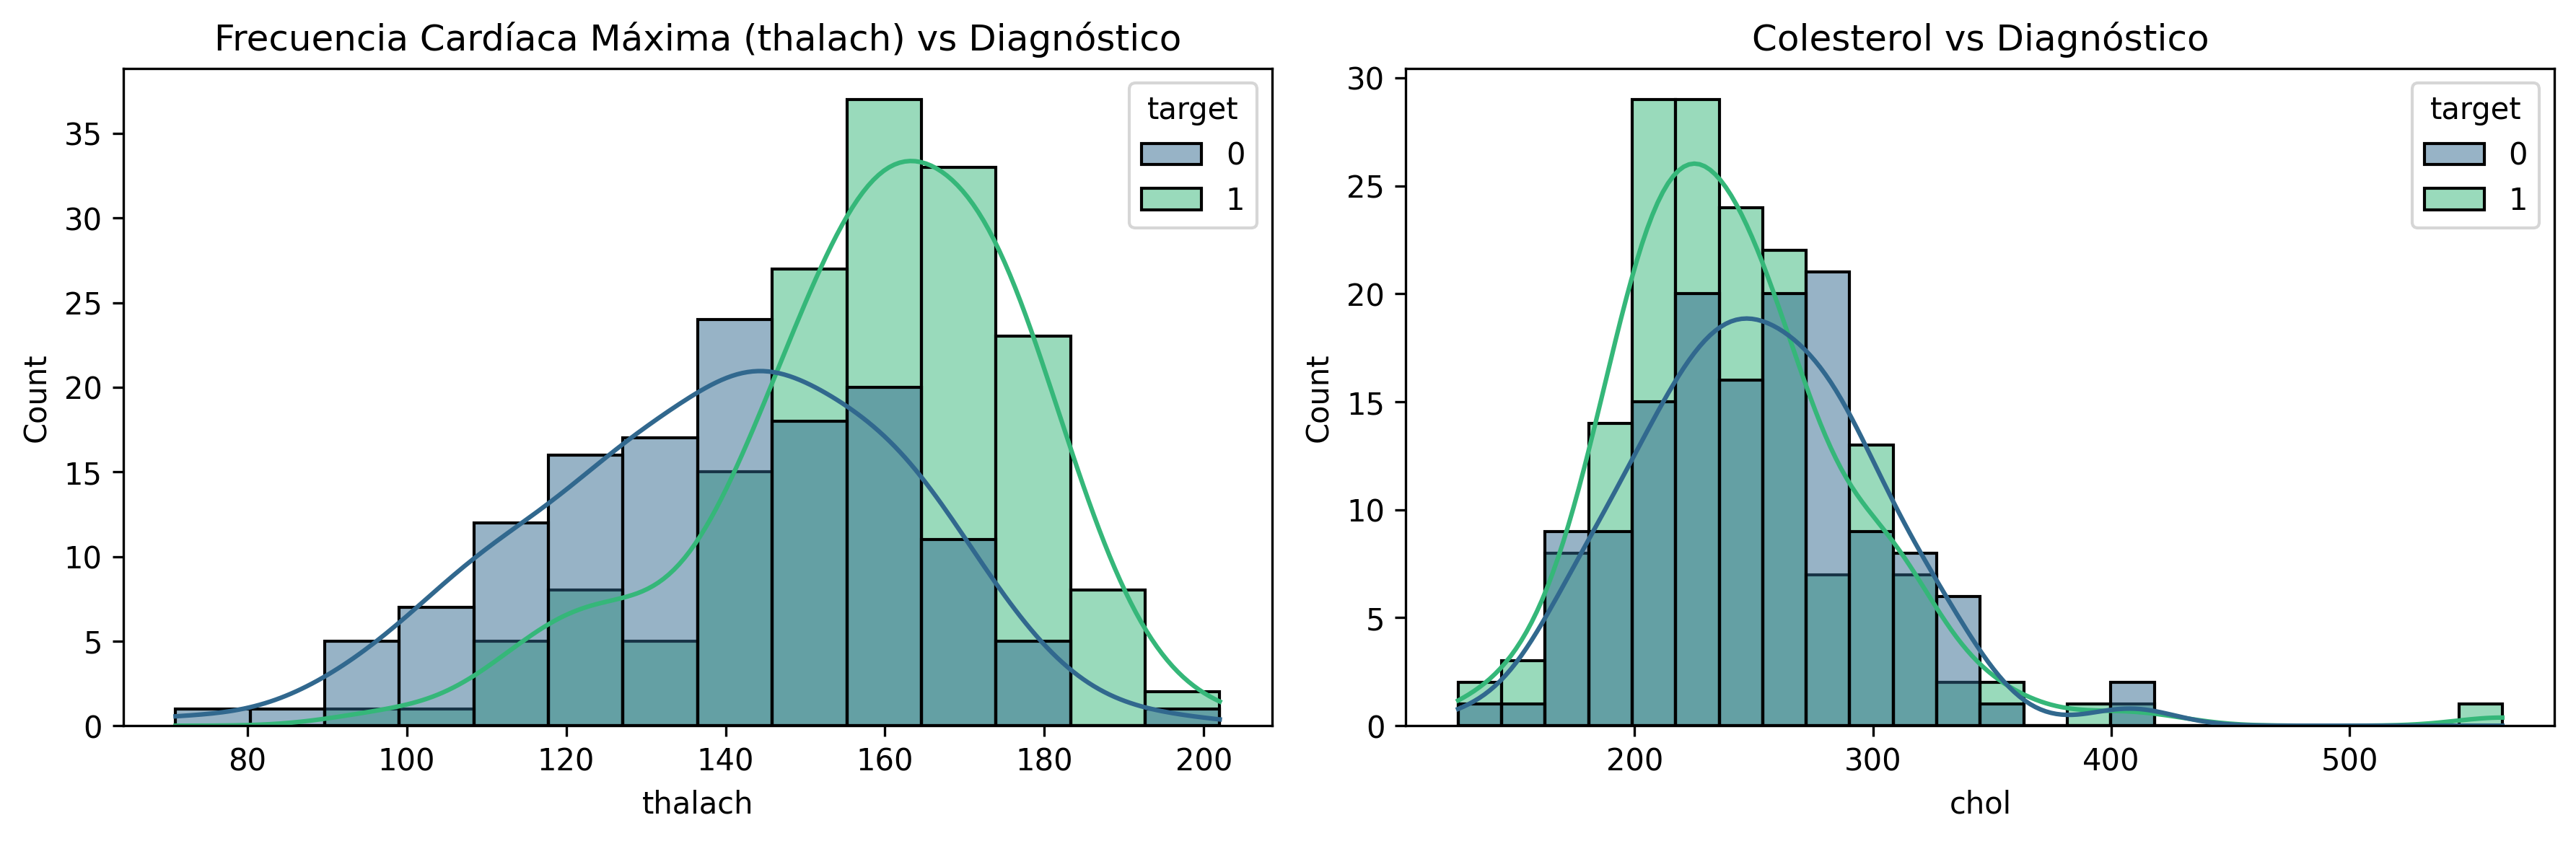
\includegraphics[width=0.45\textwidth]{Figuras/distribucion_variables.png}
    \caption{Distribución de la Frecuencia Cardíaca Máxima (izquierda) y el Colesterol (derecha) cruzados por el diagnóstico del paciente.}
    \label{fig:dist_variables}
\end{figure}

Al observar la Figura \ref{fig:dist_variables}, se revelan hallazgos cruciales:
\begin{itemize}
    \item \textbf{Frecuencia Cardíaca Máxima (\textit{thalach}):} Existe una tendencia clara en la cual los pacientes enfermos (presencia de anomalías) logran o presentan frecuencias cardíacas atípicas y superiores durante las pruebas de esfuerzo.
    \item \textbf{Colesterol:} Notamos la presencia de múltiples observaciones anómalas (outliers) que superan peligrosamente los 300 e incluso 400 mg/dl, lo que representa factores de riesgo severos fisiológicos.
\end{itemize}

%----------------------------------------------------------------------
\section{Evolución Metodológica y Matemática}
%----------------------------------------------------------------------

Con el análisis exploratorio consolidado, el diseño metodológico requirió un ajuste conceptual importante para poder discriminar efectivamente entre las dos poblaciones.

\subsection{Limitaciones de la Regresión Lineal}

Nuestro primer instinto metodológico fue plantear un modelo de Regresión Lineal Múltiple ajustado mediante Mínimos Cuadrados Ordinarios (OLS). El modelo lineal busca minimizar la suma de errores al cuadrado y se formula como $Y = \beta_0 + \sum \beta_i X_i$. Sin embargo, obtuvimos un R-cuadrado muy pobre de apenas 0.30. 

El error fundamental de este enfoque radica en la naturaleza de nuestro objetivo. El diagnóstico es un evento binario discreto (1 = Enfermo, 0 = Sano). Un modelo lineal puro no posee restricciones de límite, por lo que arroja predicciones probabilísticas teóricamente imposibles (como que un paciente tenga un $1.2$ o $-0.1$ de probabilidad de estar enfermo). 

\subsection{El Enfoque Logístico y Función Sigmoide}

Para resolver este dilema matemático, se introdujo la Regresión Logística. En lugar de predecir $Y$ directamente, la regresión logística modela el logaritmo de las probabilidades a favor (\textit{Log-Odds}):

\begin{equation}
\log\left(\frac{p}{1-p}\right) = \beta_0 + \beta_1 X_1 + \dots + \beta_k X_k
\label{eq:logodds}
\end{equation}

Posteriormente, al despejar $p$ utilizando la función \textit{Sigmoide}, se logra "aplastar" el resultado matemático para que este siempre caiga estrictamente dentro del intervalo continuo $(0, 1)$:

\begin{equation}
p_i = \frac{1}{1 + e^{-(\beta_0 + \beta_1 X_1 + \dots + \beta_k X_k)}}
\label{eq:logit}
\end{equation}

Para el modelado final, se configuró el hiperparámetro de optimización \textit{solver} en 'LBFGS' (método cuasi-Newton iterativo) y se aplicó regularización 'L2' (Ridge) para evitar que los coeficientes ($\beta$) adquirieran valores inflados debido a colinealidad.

\subsection{Interpretación de los Coeficientes y Significancia Estadística (P-value)}

El modelo logístico extrae ponderaciones ($\beta$) para cada variable clínica. En la regresión logística, un beta positivo indica que la característica aumenta el log-odds de la enfermedad, mientras que un beta negativo indica un efecto protector o inverso. Para evaluar si estas relaciones son producto del azar, utilizamos el valor $p$ (\textit{p-value}), el cual determina la significancia estadística bajo la prueba de hipótesis ($H_0$: el coeficiente es cero). Un $p < 0.05$ indica que la variable aporta información estadísticamente significativa para la predicción, permitiendo rechazar la hipótesis nula.

\begin{table}[H]
\centering
\small
\setlength{\tabcolsep}{4pt}
\begin{tabular}{lrr | lrr}
\hline
\textbf{Variable} & \textbf{Beta} & \textbf{P-value} & \textbf{Variable} & \textbf{Beta} & \textbf{P-value} \\
\hline
age     & -0.005 & 0.832 & thalach & +0.023 & \textbf{0.026}* \\
sex     & -1.758 & \textbf{0.000}* & exang   & -0.980 & \textbf{0.017}* \\
cp      & +0.860 & \textbf{0.000}* & oldpeak & -0.540 & \textbf{0.011}* \\
trestbps& -0.019 & 0.059 & slope   & +0.579 & 0.097 \\
chol    & -0.005 & 0.221 & ca      & -0.773 & \textbf{0.000}* \\
restecg & +0.466 & 0.181 & thal    & -0.900 & \textbf{0.002}* \\
\hline
\multicolumn{6}{l}{\footnotesize * Significativo al nivel del 5\% ($p < 0.05$)}
\end{tabular}
\caption{Coeficientes $\beta$ y valores $p$ extraídos del modelo logístico (vía \textit{statsmodels}).}
\label{tab:betas}
\end{table}

A partir de los resultados en la Tabla \ref{tab:betas}, se desprenden observaciones fundamentales:
\begin{itemize}
    \item \textbf{Variables Altamente Significativas:} El tipo de dolor de pecho (\textit{cp}, $p \approx 0.000$) y el número de vasos mayores (\textit{ca}, $p = 0.0001$) son los predictores más certeros. El coeficiente positivo del dolor de pecho justifica empíricamente que presentar anginas atípicas es el principal detonante o síntoma conductor hacia un diagnóstico positivo.
    \item \textbf{Frecuencia cardíaca máxima (\textit{thalach}):} Su coeficiente positivo y $p = 0.026$ corroboran estadísticamente que una frecuencia inusualmente alta durante el esfuerzo no es una anomalía aleatoria, sino un patrón que incrementa sólidamente la probabilidad del diagnóstico.
    \item \textbf{Variables No Significativas:} Interesantemente, la edad (\textit{age}, $p = 0.832$) y el colesterol en sangre (\textit{chol}, $p = 0.221$) por sí solos no superan la barrera de significancia del 5\% en el modelo multivariado. Esto implica que, aunque son factores de riesgo conocidos, cuando interactúan al mismo tiempo con la presencia de anginas (\textit{cp}) o la frecuencia cardíaca máxima (\textit{thalach}), pierden su peso predictivo directo.
\end{itemize}


%----------------------------------------------------------------------
\section{Evaluación Clínica y Resultados}
%----------------------------------------------------------------------

\subsection{Matriz de Confusión y Sensibilidad}

Para comprobar la capacidad discriminatoria del modelo logístico en un entorno de prueba de datos invisibles al entrenamiento (test set, 20\,\%), recurrimos a la Matriz de Confusión (Figura \ref{fig:matriz}). El modelo logró una Exactitud General (Accuracy) de \textbf{77.1\,\%}.

\begin{figure}[H]
    \centering
    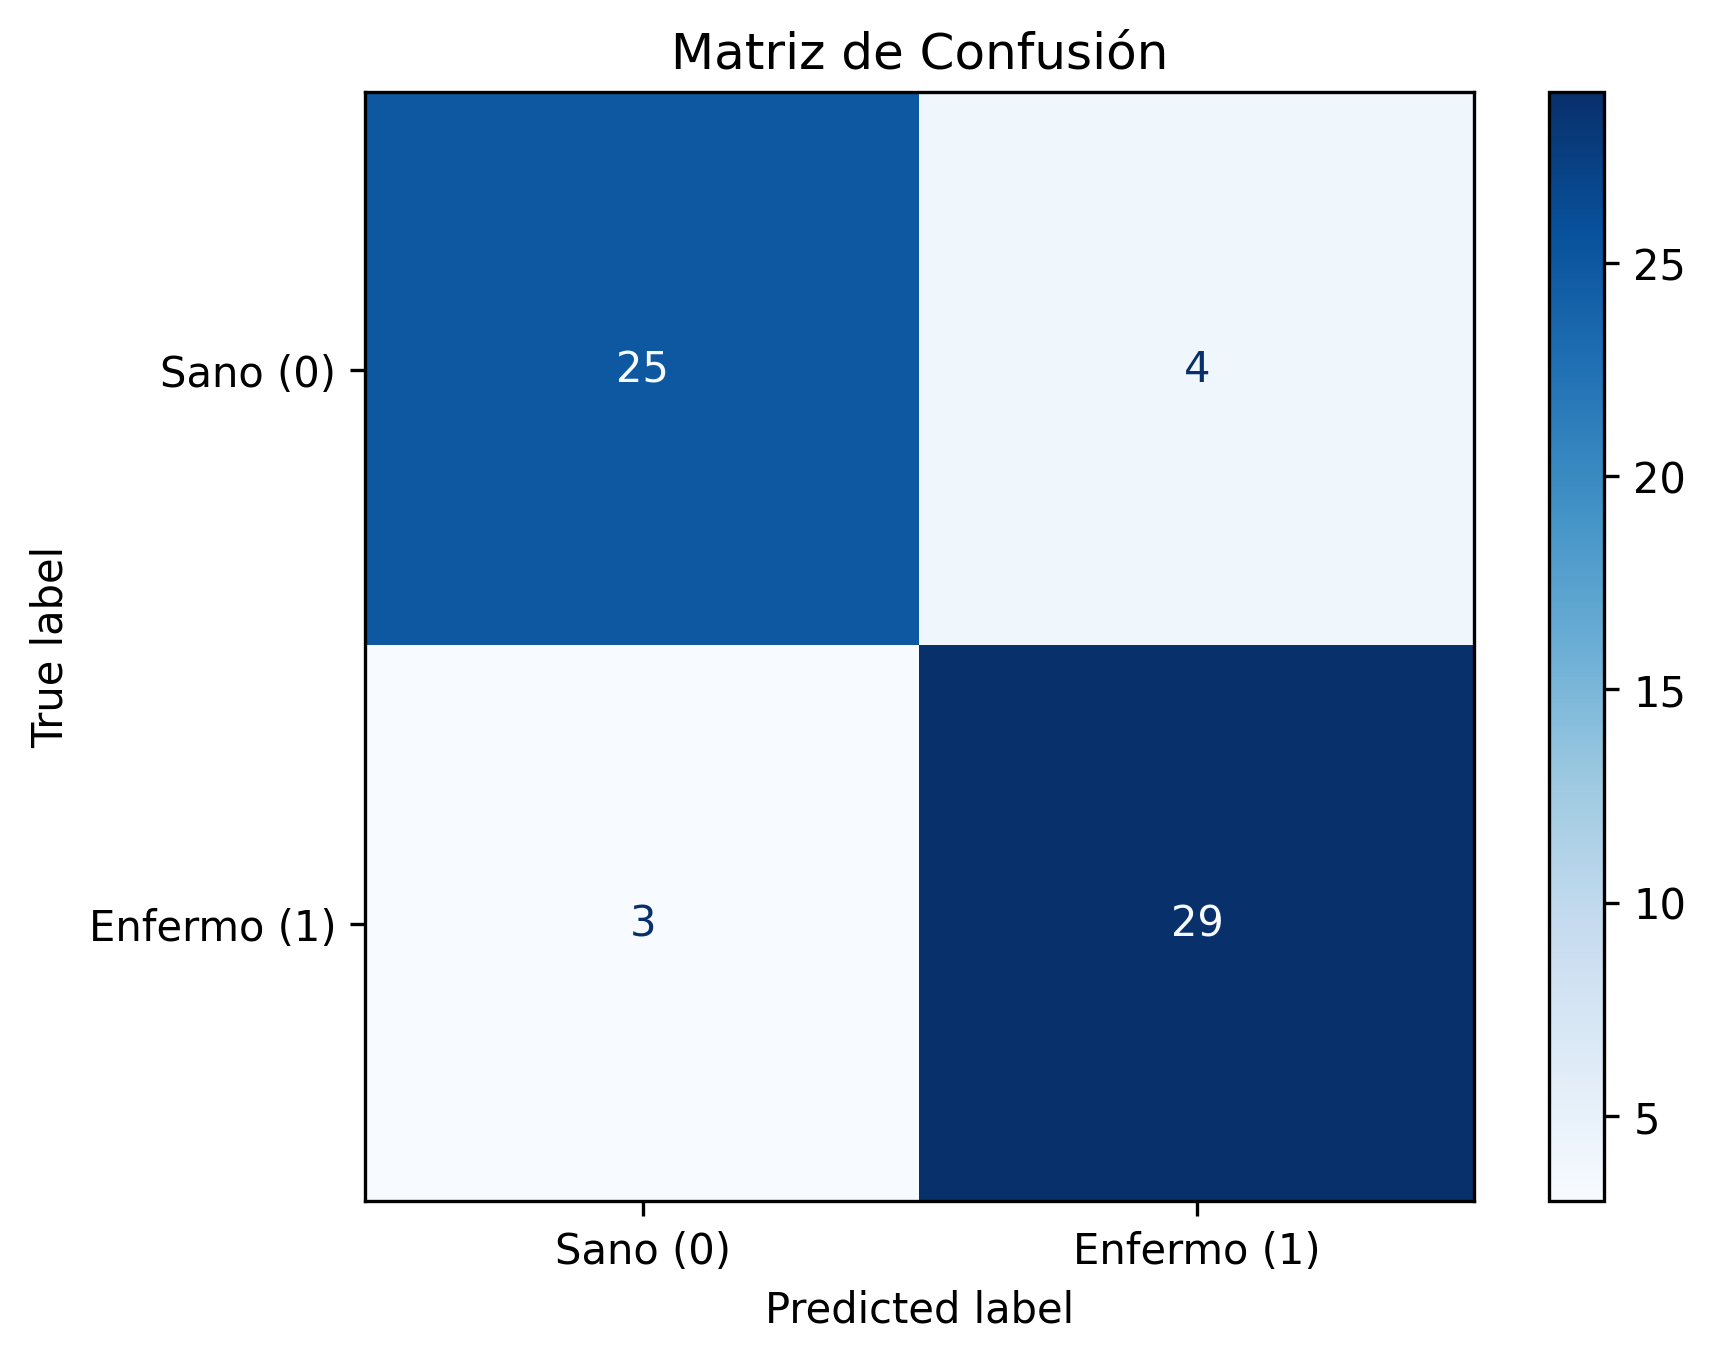
\includegraphics[width=0.45\textwidth]{Figuras/matriz_confusion.png}
    \caption{Matriz de confusión evaluada sobre el conjunto de prueba (Test). El modelo es altamente capaz de predecir correctamente la condición del paciente.}
    \label{fig:matriz}
\end{figure}

Sin embargo, en el contexto médico, la métrica de prioridad máxima es la \textbf{Sensibilidad} (Recall), es decir, la capacidad de detectar a todos los pacientes que realmente están enfermos. Nuestro algoritmo alcanzó un sólido \textbf{78.1\,\%}. Clínicamente, el sistema asume que es preferible un Falso Positivo (recomendar chequeos preventivos a un paciente sano) que cometer un Falso Negativo letal. Como se observa en la Figura \ref{fig:matriz}, el modelo limitó severamente los falsos negativos.

\subsection{Curva ROC y Área Bajo la Curva (AUC)}

Para ratificar el poder discriminativo global sin depender de un único umbral probabilístico de corte ($0.5$), evaluamos la Curva ROC (Receiver Operating Characteristic) que cruza la sensibilidad contra la tasa de falsos positivos en todo el espectro de probabilidades.

\begin{figure}[H]
    \centering
    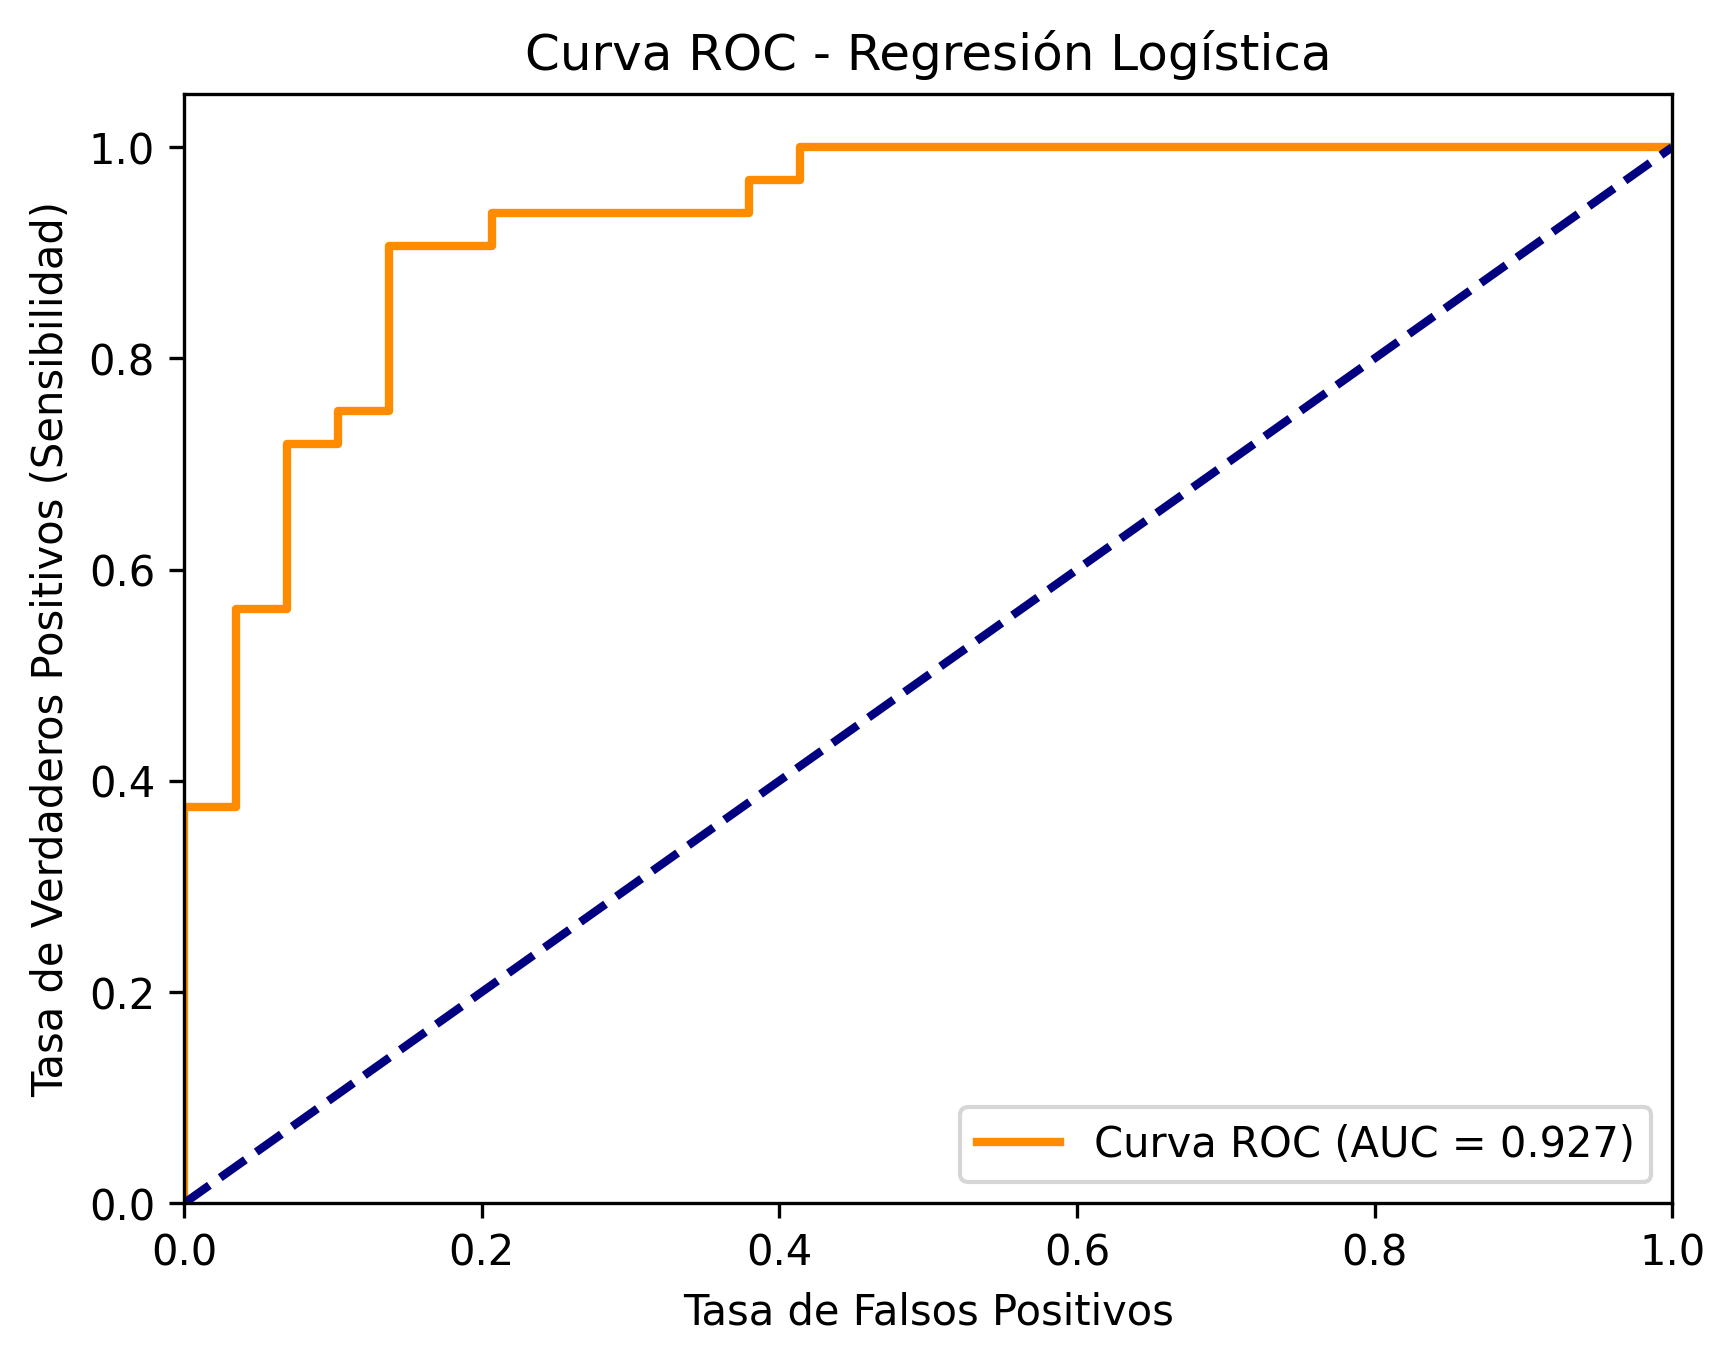
\includegraphics[width=0.45\textwidth]{Figuras/curva_roc.png}
    \caption{Curva ROC demostrando una sólida separación de clases.}
    \label{fig:roc}
\end{figure}

Nuestro clasificador logístico obtuvo un Área Bajo la Curva (AUC) de \textbf{0.838}. En las ciencias de la salud, cualquier modelo con un AUC $> 0.80$ se considera sobresaliente. Este valor confirma que el algoritmo extrae verdaderos patrones matemáticos y no se guía por azar (AUC = 0.50).

%----------------------------------------------------------------------
\section{Discusión y Conclusiones}
%----------------------------------------------------------------------

De esta investigación clínica y analítica, podemos extraer tres conclusiones principales que sientan las bases del proyecto "Healtech 1":

1. \textbf{Relevancia Clínica Empírica:} Hemos ratificado matemáticamente que las anomalías en variables fisiológicas como el tipo de angina (\textit{cp}), el esfuerzo inusual (\textit{thalach}) y el comportamiento de la perfusión coronaria funcionan como predictores primarios para la toma de decisiones clínicas.

2. \textbf{Cambio de Paradigma Metodológico:} Se demostró la falacia de aplicar algoritmos no restringidos (OLS) a clasificaciones discretas. La Regresión Logística, al operar transformando combinaciones lineales al espacio \textit{log-odds}, es la herramienta matemática adecuada para arrojar probabilidades médicas útiles.

3. \textbf{Excelencia en el Desempeño:} El modelo validado resulta sumamente robusto. Al alcanzar una sensibilidad del 78.1\,\% y un AUC de 0.838, se comprueba el gran valor añadido que proporciona el *Machine Learning* y la inferencia estadística como una segunda opinión en diagnósticos complejos, ayudando a minimizar los falsos negativos que tanto riesgo implican en la salud.

\subsection{El Paradigma del Colesterol: Una Perspectiva Clínica}

Desde una óptica médica, puede resultar contraintuitivo que un factor de riesgo tan conocido como el colesterol (\textit{chol}) no haya superado la barrera de significancia estadística en este estudio multivariado. No obstante, esto tiene una explicación clínica profunda vinculada a la diferencia entre "factores de riesgo" y "síntomas activos". El colesterol alto causa daño cardiovascular acumulativo a lo largo de décadas. Sin embargo, en el escenario agudo donde un paciente se somete a una prueba de esfuerzo, síntomas inmediatos como el dolor de pecho (\textit{cp}) o una respuesta mecánica inusual del corazón (\textit{thalach}) evidencian un daño estructural ya instaurado. Una vez el algoritmo detecta la presencia del síntoma activo que "delata" la enfermedad, el nivel subyacente de colesterol deja de aportar información predictiva diferencial inmediata. Adicionalmente, es altamente probable que muchos pacientes en esta cohorte hospitalaria (tanto los enfermos como los sanos) presenten perfiles lipídicos alterados por la edad, o contrariamente, "artificialmente" controlados por el uso previo de estatinas, lo que neutraliza su poder como discriminador directo en urgencias frente a las mediciones fisiológicas dinámicas.

\subsection{Trabajo Futuro (Healtech 2)}

Como evolución natural del proyecto, nos hemos propuesto atacar el porcentaje de error remanente explorando algoritmos de ensamble y métodos basados en árboles, tales como \textit{Random Forests} o \textit{Gradient Boosting}, los cuales podrían capturar interacciones inter-paramétricas no lineales dentro del perfil clínico integral del paciente.


%----------------------------------------------------------------------
\bibliographystyle{apalike}
%\bibliography{Bibliografia} % Descomentar si se incluye archivo BibTeX
%----------------------------------------------------------------------

\end{document}